\def\AnswerOnly{1}
% !TeX program = xelatex
% 由 教学课件/习题课模板/习题课模板.tex 复制并填充。
% 原图基础知识提取为挖空陈述与表格；每frame前保留照片来源。
% 默认首屏挖空、次屏显答案。定义 BlankOnly 或 AnswerOnly 可输出单态版本。
\documentclass[UTF8,10pt,aspectratio=169]{ctexbeamer}
\usepackage{amsmath,amssymb,tikz}
\usetikzlibrary{calc,arrows.meta,positioning}
\usepackage{newtxtext,newtxmath}
\usetheme{default}\usecolortheme{default}\usefonttheme{serif}
\setbeamertemplate{navigation symbols}{}
\setbeamertemplate{footline}[frame number]
\setbeamersize{text margin left=0.75cm,text margin right=0.75cm}
\setbeamerfont{frametitle}{size=\Large,series=\bfseries}
\setbeamerfont{itemize/enumerate body}{size=\large}
\setbeamerfont{itemize/enumerate subbody}{size=\large}
\AtBeginEnvironment{frame}{\large}
\setlength{\abovedisplayskip}{6pt}\setlength{\belowdisplayskip}{6pt}
\definecolor{AnswerBlue}{RGB}{27,91,163}
\newsavebox{\GapMeasure}
\newcommand{\Gap}[2]{%
  \begingroup\sbox{\GapMeasure}{\strut#2}%
  \ifdim\wd\GapMeasure>#1\relax
    \PackageWarning{cloze}{Answer wider than blank: \detokenize{#2}}%
  \fi
  \mbox{\underline{\makebox[#1][c]{\strut\vphantom{#2}%
    \ifdefined\BlankOnly\phantom{#2}%
    \else\ifdefined\AnswerOnly\textcolor{AnswerBlue}{#2}%
    \else\alt<2->{\textcolor{AnswerBlue}{#2}}{\phantom{#2}}%
    \fi\fi}}}%
  \endgroup}
\newcommand{\Reveal}[1]{%
  \par\vspace{0.23cm}\noindent
  \ifdefined\BlankOnly\phantom{\parbox{\linewidth}{#1}}%
  \else\ifdefined\AnswerOnly\parbox{\linewidth}{#1}%
  \else\uncover<2->{\parbox{\linewidth}{#1}}\fi\fi\par}
\newcommand{\Session}[2]{\section{#2}\begin{frame}\begin{center}\vspace{0.7cm}{\Large 第#1节晚自习}\par\vspace{0.5cm}{\LARGE\bfseries #2}\par\vspace{0.6cm}先填写横线\qquad 再点击核对\end{center}\end{frame}}
\begin{document}
\begin{frame}
\begin{center}
{\LARGE\bfseries 高一数学期中}\par\vspace{0.3cm}
{\LARGE\bfseries 基础知识挖空复习}\par\vspace{0.65cm}
集合与逻辑\quad 不等式\quad 函数\quad 指数函数\par\vspace{0.6cm}
看白板填空\qquad 点击核对答案
\end{center}
\end{frame}
\begin{frame}[t]{填写与核对}
\begin{enumerate}
\item 看清句子、公式或表格，在横线处填写知识内容。
\item 先独立写，再点击显示蓝色答案。
\item 对照答案，补齐漏掉的符号、条件和端点。
\end{enumerate}
\par\vspace{0.7cm}
\textbf{按页号记录；需要时停留在挖空页，完成后再核对。}
\end{frame}

\Session{一}{集合与逻辑}
% 来源：微信图片_20261112170218_485_20.jpg；知识点一：元素与集合的含义、元素的性质。
\begin{frame}[t]{集合的含义与元素的性质}
\begin{enumerate}
\item 一般地，把\Gap{2.5cm}{研究对象}统称为元素。
\item 把一些元素组成的\Gap{1.8cm}{总体}叫做集合，简称\Gap{1cm}{集}。
\item 某个对象是否属于一个已确定的集合，是确定的，这体现元素的\Gap{2cm}{确定性}。
\item 集合中的元素不能重复，这体现元素的\Gap{2cm}{互异性}。
\item 集合中的元素没有先后顺序，这体现元素的\Gap{2cm}{无序性}。
\end{enumerate}
\Reveal{两个集合的元素完全相同，这两个集合就相等。}
\end{frame}

% 来源：微信图片_20261112170218_485_20.jpg；知识点二：元素与集合的关系、常用数集。
\begin{frame}[t]{元素与集合的关系、常用数集}
\begin{itemize}
\item $a$ 是集合 $A$ 的元素，记作\Gap{1.8cm}{$a\in A$}；不是其中的元素，记作\Gap{1.8cm}{$a\notin A$}。
\end{itemize}
\renewcommand{\arraystretch}{1.6}
\begin{center}
\begin{tabular}{c|c@{\qquad}c|c}
数集&符号&数集&符号\\ \hline
非负整数集&\Gap{1.1cm}{$\mathbb N$}&正整数集&\Gap{1.1cm}{$\mathbb N^*$}\\
整数集&\Gap{1.1cm}{$\mathbb Z$}&有理数集&\Gap{1.1cm}{$\mathbb Q$}\\
实数集&\Gap{1.1cm}{$\mathbb R$}&&
\end{tabular}
\end{center}
\Reveal{非负整数集也叫自然数集；$0\in\mathbb N$，$0\notin\mathbb N^*$。}
\end{frame}

% 来源：微信图片_20261112170218_485_20.jpg；知识点三：集合的表示方法。
\begin{frame}[t]{集合的表示方法}
\begin{enumerate}
\item \textbf{列举法：}把集合的所有元素\Gap{2cm}{一一列举}出来，并用花括号\Gap{1.1cm}{$\{\ \}$}括起来。
\item \textbf{描述法：}把集合中所有具有\Gap{2.3cm}{共同特征}$p(x)$ 的元素 $x$ 所组成的集合表示为
\[
\Gap{5.6cm}{$\{x\mid p(x)\}$}.
\]
\item 通常用小写拉丁字母表示\Gap{1.4cm}{元素}，用大写拉丁字母表示\Gap{1.4cm}{集合}。
\end{enumerate}
\Reveal{描述法先看元素是什么，再看它满足什么条件。}
\end{frame}

% 来源：微信图片_20261112170221_490_20.jpg；知识点一：子集、集合相等。
\begin{frame}[t]{子集与集合相等}
\begin{enumerate}
\item 如果集合 $A$ 中\Gap{1.8cm}{任意一个}元素都是集合 $B$ 中的元素，就称 $A$ 是 $B$ 的\Gap{1.5cm}{子集}。
\item 记作 $A\subseteq B$（或 $B\supseteq A$）。
\item 任何一个集合都是它本身的子集，即\Gap{2cm}{$A\subseteq A$}。
\item 若 $A\subseteq B$ 且 $B\subseteq C$，则\Gap{2cm}{$A\subseteq C$}。
\item 若 $A\subseteq B$ 且 $B\subseteq A$，则\Gap{2cm}{$A=B$}。
\end{enumerate}
\Reveal{$\in$ 表示元素与集合的关系；$\subseteq$ 表示集合与集合的关系。}
\end{frame}

% 来源：微信图片_20261112170221_490_20.jpg；知识点一真子集、知识点二空集。
\begin{frame}[t]{真子集与空集}
\begin{enumerate}
\item 若 $A\subseteq B$，且存在元素 $x\in B$、$x\notin A$，则称 $A$ 是 $B$ 的\Gap{1.7cm}{真子集}，记作\Gap{2cm}{$A\subsetneq B$}。
\item 不含\Gap{1.8cm}{任何元素}的集合叫做空集，记作\Gap{1.3cm}{$\varnothing$}。
\item 空集是任何集合的\Gap{1.3cm}{子集}；若 $A\ne\varnothing$，则空集是 $A$ 的\Gap{1.7cm}{真子集}。
\item 空集只有\Gap{1.2cm}{一个}子集，就是它本身。
\end{enumerate}
\Reveal{$\varnothing$ 是集合，$0$ 是实数；$\{0\}$ 中有一个元素，不能与空集混同。}
\end{frame}

% 来源：微信图片_20261112170225_491_20.jpg；知识点一：并集。
\begin{frame}[t]{并集}
\begin{itemize}
\item 由所有属于集合 $A$\Gap{1cm}{或}属于集合 $B$ 的元素组成的集合，称为 $A$ 与 $B$ 的并集。
\item 记作\Gap{2cm}{$A\cup B$}，读作\Gap{2cm}{$A$ 并 $B$}。
\item 符号表示：
\[
\Gap{9cm}{$A\cup B=\{x\mid x\in A\text{ 或 }x\in B\}$}.
\]
\end{itemize}
\begin{center}
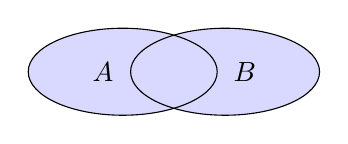
\begin{tikzpicture}[x=1cm,y=0.65cm]
\fill[blue!15](-0.65,0)ellipse(1.2 and 0.85);
\fill[blue!15](0.65,0)ellipse(1.2 and 0.85);
\draw(-0.65,0)ellipse(1.2 and 0.85);\draw(0.65,0)ellipse(1.2 and 0.85);
\node at(-0.9,0){$A$};\node at(0.9,0){$B$};
\end{tikzpicture}
\end{center}
\Reveal{“或”包含同时属于两个集合的情形；重复元素只写一次。}
\end{frame}

% 来源：微信图片_20261112170225_491_20.jpg；知识点二：交集。
\begin{frame}[t]{交集}
\begin{itemize}
\item 由所有属于集合 $A$\Gap{1cm}{且}属于集合 $B$ 的元素组成的集合，称为 $A$ 与 $B$ 的交集。
\item 记作\Gap{2cm}{$A\cap B$}，读作\Gap{2cm}{$A$ 交 $B$}。
\item 符号表示：
\[
\Gap{9cm}{$A\cap B=\{x\mid x\in A\text{ 且 }x\in B\}$}.
\]
\end{itemize}
\begin{center}
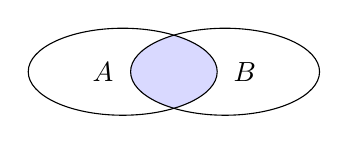
\begin{tikzpicture}[x=1cm,y=0.65cm]
\begin{scope}\clip(-0.65,0)ellipse(1.2 and 0.85);\fill[blue!15](0.65,0)ellipse(1.2 and 0.85);\end{scope}
\draw(-0.65,0)ellipse(1.2 and 0.85);\draw(0.65,0)ellipse(1.2 and 0.85);
\node at(-0.9,0){$A$};\node at(0.9,0){$B$};
\end{tikzpicture}
\end{center}
\Reveal{交集只保留共有元素；没有共有元素时，交集为空集。}
\end{frame}

% 来源：微信图片_20261112170227_492_20.jpg；全集、补集的定义。
\begin{frame}[t]{全集与补集}
\begin{enumerate}
\item 含有所研究问题中涉及的\Gap{2cm}{所有元素}的集合叫做全集，通常记作 $U$。
\item 设 $A\subseteq U$。由全集 $U$ 中\Gap{2.2cm}{不属于}集合 $A$ 的所有元素组成的集合，称为 $A$ 相对于 $U$ 的补集。
\item 补集记作\Gap{2cm}{$\complement_U A$}，即
\[
\Gap{9.5cm}{$\complement_U A=\{x\mid x\in U\text{ 且 }x\notin A\}$}.
\]
\end{enumerate}
\Reveal{全集不一定是实数集；先确定全集，再求补集。}
\end{frame}

% 来源：微信图片_20261112170227_492_20.jpg；补集的性质（1）—（5）。
\begin{frame}[t]{补集的性质}
设 $A,B\subseteq U$，则
\[
\begin{aligned}
A\cup(\complement_U A)&=\Gap{1.8cm}{$U$},
&A\cap(\complement_U A)&=\Gap{1.8cm}{$\varnothing$},\\[0.45em]
\complement_U U&=\Gap{1.8cm}{$\varnothing$},
&\complement_U\varnothing&=U,\\[0.45em]
\complement_U(\complement_U A)&=\Gap{1.8cm}{$A$}.&&
\end{aligned}
\]
\[
(\complement_U A)\cap(\complement_U B)=\Gap{4.5cm}{$\complement_U(A\cup B)$},
\]
\[
(\complement_U A)\cup(\complement_U B)=\Gap{4.5cm}{$\complement_U(A\cap B)$}.
\]
\Reveal{取交、并的补集时，交与并要互换，每个集合也要取补。}
\end{frame}

% 来源：微信图片_20261112170230_493_20.jpg；充分条件与必要条件。
\begin{frame}[t]{充分条件与必要条件}
\begin{enumerate}
\item “若 $p$，则 $q$”为真命题，记作\Gap{2.2cm}{$p\Rightarrow q$}。
\item 此时，$p$ 是 $q$ 的\Gap{1.8cm}{充分}条件，$q$ 是 $p$ 的\Gap{1.8cm}{必要}条件。
\item “若 $p$，则 $q$”为假命题，记作\Gap{2.2cm}{$p\nRightarrow q$}。
\item 此时，$p$ 不是 $q$ 的\Gap{1.8cm}{充分}条件，$q$ 不是 $p$ 的\Gap{1.8cm}{必要}条件。
\end{enumerate}
\Reveal{认清“谁是谁的条件”；箭头起点为终点的充分条件，终点为起点的必要条件。}
\end{frame}

% 来源：微信图片_20261112170234_494_20.jpg；充要条件、四种条件关系。
\begin{frame}[t]{四种条件关系}
\renewcommand{\arraystretch}{1.8}
\begin{center}
\begin{tabular}{c|c}
推导关系&$p$ 是 $q$ 的什么条件\\ \hline
$p\Rightarrow q$，$q\nRightarrow p$&\Gap{4cm}{充分不必要条件}\\
$q\Rightarrow p$，$p\nRightarrow q$&\Gap{4cm}{必要不充分条件}\\
$p\Rightarrow q$，$q\Rightarrow p$&\Gap{4cm}{充要条件}\\
$p\nRightarrow q$，$q\nRightarrow p$&\Gap{4.6cm}{既不充分也不必要条件}
\end{tabular}
\end{center}
两个方向都能推出时，记作\Gap{2.5cm}{$p\Leftrightarrow q$}，$p$ 与 $q$ 互为\Gap{2cm}{充要}条件。
\end{frame}

% 来源：微信图片_20261112170234_494_20.jpg；从集合角度看充分、必要条件。
\begin{frame}[t]{从集合关系看条件关系}
在相同研究范围内，设
\[
A=\{x\mid p(x)\},\qquad B=\{x\mid q(x)\}.
\]
\renewcommand{\arraystretch}{1.7}
\begin{center}
\begin{tabular}{c|c}
集合关系&$p$ 是 $q$ 的什么条件\\ \hline
$A\subsetneq B$&\Gap{4cm}{充分不必要条件}\\
$B\subsetneq A$&\Gap{4cm}{必要不充分条件}\\
$A=B$&\Gap{4cm}{充要条件}\\
$A\nsubseteq B$ 且 $B\nsubseteq A$&\Gap{4.6cm}{既不充分也不必要条件}
\end{tabular}
\end{center}
\Reveal{先判断集合包含关系，再确定推导方向。}
\end{frame}

% 来源：微信图片_20261112170237_495_20.jpg；全称量词与存在量词及命题一般形式。
\begin{frame}[t]{全称量词与存在量词}
\begin{enumerate}
\item 短语“\Gap{1.5cm}{所有}”“\Gap{2.1cm}{任意一个}”叫作全称量词，符号为\Gap{1.1cm}{$\forall$}。
\item “对 $M$ 中的每个元素 $x$，$p(x)$ 成立”，符号形式为
\[
\Gap{5.3cm}{$\forall x\in M,\ p(x)$}.
\]
\item 短语“\Gap{1.8cm}{存在一个}”“\Gap{1.8cm}{至少一个}”叫作存在量词，符号为\Gap{1.1cm}{$\exists$}。
\item “存在 $M$ 中的元素 $x$，$p(x)$ 成立”，符号形式为
\[
\Gap{5.3cm}{$\exists x\in M,\ p(x)$}.
\]
\end{enumerate}
\end{frame}

% 来源：微信图片_20261112170240_496_20.jpg；命题否定、全称量词命题的否定。
\begin{frame}[t]{命题的否定与全称命题的否定}
\begin{enumerate}
\item 一个命题和它的否定不能同时为\Gap{1.2cm}{真}，也不能同时为\Gap{1.2cm}{假}，只能\Gap{2cm}{一真一假}。
\item 原命题：$\forall x\in M,\ p(x)$。其否定为
\[
\Gap{6.2cm}{$\exists x\in M,\ \neg p(x)$}.
\]
\item 全称量词命题的否定是\Gap{2.4cm}{存在量词}命题。
\item 原命题为真，其否定为\Gap{1.2cm}{假}；原命题为假，其否定为\Gap{1.2cm}{真}。
\end{enumerate}
\Reveal{$\neg p(x)$ 表示“$p(x)$ 不成立”；否定时变量的范围 $M$ 保持不变。}
\end{frame}

% 来源：微信图片_20261112170243_497_20.jpg；存在量词命题的否定。兼据496命题否定的微提醒。
\begin{frame}[t]{存在命题的否定}
\begin{enumerate}
\item 原命题：$\exists x\in M,\ p(x)$。其否定为
\[
\Gap{6.2cm}{$\forall x\in M,\ \neg p(x)$}.
\]
\item 存在量词命题的否定是\Gap{2.4cm}{全称量词}命题。
\item 写量词命题的否定时，要\Gap{2cm}{改变量词}，并\Gap{2cm}{否定结论}。
\item 写量词命题的否定时，否定\Gap{1.4cm}{结论}，保留\Gap{2cm}{变量范围}。
\end{enumerate}
\Reveal{全称与存在互换；“不成立”要覆盖原命题的完整结论。}
\end{frame}

\Session{二}{不等式与函数性质}
% PART: INEQUALITIES
% 来源：微信图片_20261112170246_498_20.jpg；实数的大小比较的基本事实。
\begin{frame}[t]{实数大小：作差看正负}
\large
设 $a,b\in\mathbb R$，则
\begin{enumerate}
\item 如果 $a-b$ 是\Gap{1.6cm}{正数}，那么 $a>b$。
\item 如果 $a-b$ \Gap{1.6cm}{等于零}，那么 $a=b$。
\item 如果 $a-b$ 是\Gap{1.6cm}{负数}，那么 $a<b$。
\end{enumerate}
\Reveal{作差以后判断差的正负；不能只看某一项的符号。}
\end{frame}

% 来源：微信图片_20261112170246_498_20.jpg；等式的性质。
\begin{frame}[t]{等式的五条基本性质}
\large
\begin{enumerate}
\item 若 $a=b$，则\Gap{2cm}{$b=a$}。
\item 若 $a=b$，$b=c$，则\Gap{2cm}{$a=c$}。
\item 若 $a=b$，则 $a\pm c=$\Gap{2cm}{$b\pm c$}。
\item 若 $a=b$，则 $ac=$\Gap{2cm}{$bc$}。
\item 若 $a=b$，且\Gap{1.8cm}{$c\ne0$}，则 $\dfrac ac=\dfrac bc$。
\end{enumerate}
\Reveal{等式两边同除一个数时，要先排除除数为零。}
\end{frame}

% 来源：微信图片_20261112170246_498_20.jpg；不等式性质表。
\begin{frame}[t]{不等式的性质}
\large
\begin{enumerate}
\item $a>b\iff$\Gap{1.8cm}{$b<a$}；$a>b,\ b>c\Rightarrow$\Gap{1.8cm}{$a>c$}。
\item $a>b\iff$\Gap{3.8cm}{$a+c>b+c$}。
\item $a>b,\ c>0\Rightarrow ac$\Gap{0.7cm}{$>$}$bc$；
\par $a>b,\ c<0\Rightarrow ac$\Gap{0.7cm}{$<$}$bc$。
\item $a>b,\ c>d\Rightarrow$\Gap{3.8cm}{$a+c>b+d$}。
\item $a>b>0,\ c>d>0\Rightarrow$\Gap{2.8cm}{$ac>bd$}。
\item $a>b>0,\ n\in\mathbb N,\ n\ge2\Rightarrow$\Gap{2.8cm}{$a^n>b^n$}。
\end{enumerate}
\Reveal{乘除前判断符号；符号未知时不能直接乘除。}
\end{frame}

% 来源：微信图片_20261112170249_499_20.jpg；重要不等式、基本不等式与平均数。
\begin{frame}[t]{基本不等式：公式与等号}
\large
\begin{enumerate}
\item 若 $a,b\in\mathbb R$，则 $a^2+b^2$\Gap{0.8cm}{$\ge$}$2ab$，等号成立当且仅当\Gap{1.8cm}{$a=b$}。
\item 若 $a>0,b>0$，则 $\sqrt{ab}$\Gap{0.8cm}{$\le$}$\dfrac{a+b}{2}$，等号成立当且仅当\Gap{1.8cm}{$a=b$}。
\item $\dfrac{a+b}{2}$ 叫作正数 $a,b$ 的\Gap{2.6cm}{算术平均数}；$\sqrt{ab}$ 叫作它们的\Gap{2.6cm}{几何平均数}。
\item 两个正数的算术平均数\Gap{1.6cm}{不小于}它们的几何平均数。
\end{enumerate}
\Reveal{使用含根号的公式时，先检查所比较的量满足条件。}
\end{frame}

% 来源：微信图片_20261112170249_499_20.jpg；基本不等式与最值、“一正二定三相等”。
\begin{frame}[t]{基本不等式与最值}
\large
已知 $x,y$ 都是正数。
\begin{enumerate}
\item 若 $xy=P$ 为定值，则当\Gap{1.8cm}{$x=y$}时，$x+y$ 有最小值\Gap{2cm}{$2\sqrt P$}。
\item 若 $x+y=S$ 为定值，则当\Gap{1.8cm}{$x=y$}时，$xy$ 有最大值\Gap{2cm}{$\dfrac{S^2}{4}$}。
\item “一正”：比较量满足\Gap{1.8cm}{正数条件}。
\item “二定”：化不等式的一边为\Gap{1.6cm}{定值}。
\item “三相等”：等号成立的条件必须\Gap{2.1cm}{能够取到}。
\end{enumerate}
\Reveal{三项检查缺一不可；给出上界或下界以后，还要验证等号可取。}
\end{frame}

% 来源：微信图片_20261112170252_500_20.jpg；一元二次不等式定义、一般形式与二次函数零点。
\begin{frame}[t]{一元二次不等式与二次函数零点}
\large
\begin{enumerate}
\item 只含有\Gap{1cm}{一个}未知数，并且未知数的最高次数是\Gap{1cm}{二}的不等式，叫作一元二次不等式。
\item 一般形式为 $ax^2+bx+c>0$ 或 $ax^2+bx+c<0$，其中 $a,b,c$ 为常数，且\Gap{1.6cm}{$a\ne0$}。
\item 使\Gap{3.4cm}{$ax^2+bx+c=0$}的实数 $x$，叫作二次函数 $y=ax^2+bx+c$ 的\Gap{1.2cm}{零点}。
\item 判别式为 $\Delta=$\Gap{2.5cm}{$b^2-4ac$}。
\end{enumerate}
\Reveal{零点是自变量的值，不是图像上的点；函数、方程和不等式要结合图像理解。}
\end{frame}

% 来源：微信图片_20261112170252_500_20.jpg；“三个二次”关系表，Delta>0。
\begin{frame}[t]{二次不等式：$a>0$，$\Delta>0$}
\large
方程 $ax^2+bx+c=0$ 有\Gap{4.2cm}{两个不相等的实根} $x_1<x_2$。
\begin{columns}[c,onlytextwidth]
\begin{column}{0.28\textwidth}\centering
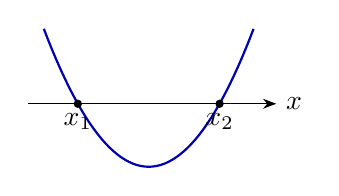
\begin{tikzpicture}[x=0.9cm,y=0.8cm,>=Stealth]
\draw[->](-1.7,0)--(1.8,0) node[right]{$x$};
\draw[blue!70!black,thick,domain=-1.48:1.48,samples=55]plot(\x,{\x*\x-1});
\fill(-1,0)circle(1.5pt)node[below]{$x_1$};
\fill(1,0)circle(1.5pt)node[below]{$x_2$};
\end{tikzpicture}
\end{column}
\begin{column}{0.68\textwidth}
$ax^2+bx+c>0$ 的解集为\par\vspace{0.12cm}
\Gap{5.8cm}{$(-\infty,x_1)\cup(x_2,+\infty)$}。\par\vspace{0.35cm}
$ax^2+bx+c<0$ 的解集为\par\vspace{0.12cm}
\Gap{3.8cm}{$(x_1,x_2)$}。
\end{column}
\end{columns}
\Reveal{开口向上，两根外侧为正、两根之间为负；不等号含等号时补入相应实根。}
\end{frame}

% 来源：微信图片_20261112170252_500_20.jpg；“三个二次”关系表，Delta=0；补齐非严格不等式的边界。
\begin{frame}[t]{二次不等式：$a>0$，$\Delta=0$}
\large
方程有两个相等的实根 $x_1=x_2=$\Gap{2.1cm}{$-\dfrac{b}{2a}$}，记为 $x_0$。
\begin{columns}[c,onlytextwidth]
\begin{column}{0.28\textwidth}\centering
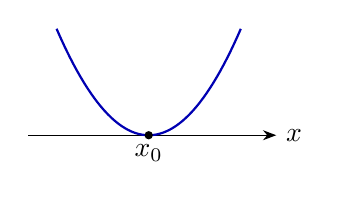
\begin{tikzpicture}[x=0.9cm,y=0.8cm,>=Stealth]
\draw[->](-1.7,0)--(1.8,0)node[right]{$x$};
\draw[blue!70!black,thick,domain=-1.3:1.3,samples=55]plot(\x,{\x*\x});
\fill(0,0)circle(1.5pt)node[below]{$x_0$};
\end{tikzpicture}
\end{column}
\begin{column}{0.68\textwidth}
\begin{tabular}{@{}ll@{}}
不等式 & 解集\\[0.15cm]
$ax^2+bx+c>0$ & \Gap{3cm}{$\mathbb R\setminus\{x_0\}$}\\[0.15cm]
$ax^2+bx+c<0$ & \Gap{3cm}{$\varnothing$}\\[0.15cm]
$ax^2+bx+c\ge0$ & \Gap{3cm}{$\mathbb R$}\\[0.15cm]
$ax^2+bx+c\le0$ & \Gap{3cm}{$\{x_0\}$}
\end{tabular}
\end{column}
\end{columns}
\Reveal{图像与 $x$ 轴相切；函数值等于零只在 $x=x_0$ 处发生。}
\end{frame}

% 来源：微信图片_20261112170252_500_20.jpg；“三个二次”关系表，Delta<0。
\begin{frame}[t]{二次不等式：$a>0$，$\Delta<0$}
\large
方程 $ax^2+bx+c=0$\Gap{2.4cm}{没有实数根}，图像与 $x$ 轴\Gap{1.8cm}{没有交点}。
\begin{columns}[c,onlytextwidth]
\begin{column}{0.28\textwidth}\centering
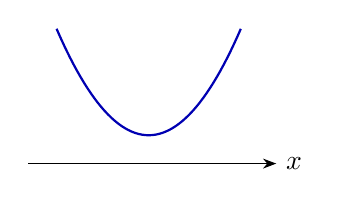
\begin{tikzpicture}[x=0.9cm,y=0.8cm,>=Stealth]
\draw[->](-1.7,0)--(1.8,0)node[right]{$x$};
\draw[blue!70!black,thick,domain=-1.3:1.3,samples=55]plot(\x,{\x*\x+0.45});
\end{tikzpicture}
\end{column}
\begin{column}{0.68\textwidth}
$ax^2+bx+c>0$ 的解集为\Gap{2cm}{$\mathbb R$}。\par\vspace{0.35cm}
$ax^2+bx+c<0$ 的解集为\Gap{2cm}{$\varnothing$}。\par\vspace{0.35cm}
对任意 $x\in\mathbb R$，函数值始终\Gap{1.6cm}{大于零}。
\end{column}
\end{columns}
\Reveal{上述三页均以 $a>0$ 为前提；$a<0$ 时可先同乘 $-1$，同时改变不等号方向。}
\end{frame}

% PART: FUNCTIONS
% 来源：微信图片_20261112170255_501_20.jpg；函数的概念、记法、定义域、函数值、值域。
\begin{frame}[t]{函数的概念}
\large
设 $A,B$ 是\Gap{3cm}{非空的实数集}。对于集合 $A$ 中的\Gap{1.7cm}{任意一个}数 $x$，按照确定的对应关系 $f$，在集合 $B$ 中都有\Gap{2cm}{唯一确定}的数 $y$ 与它对应，则称 $f$ 为从 $A$ 到 $B$ 的函数，记作 $y=f(x)$，$x\in A$。
\par\vspace{0.35cm}
\begin{enumerate}
\item $x$ 叫作\Gap{1.6cm}{自变量}；$x$ 的取值范围 $A$ 叫作函数的\Gap{1.6cm}{定义域}。
\item 与 $x$ 对应的 $y$ 叫作\Gap{1.6cm}{函数值}。
\item 函数值的集合叫作函数的\Gap{1.6cm}{值域}。
\end{enumerate}
\Reveal{“任意一个”保证输入不遗漏；“唯一确定”保证同一输入只有一个输出。}
\end{frame}

% 来源：微信图片_20261112170255_501_20.jpg；同一个函数及定义域、对应关系、值域的关系。
\begin{frame}[t]{同一个函数与函数要素}
\large
\begin{enumerate}
\item 如果两个函数的\Gap{1.8cm}{定义域}相同，并且\Gap{2.2cm}{对应关系}完全一致，那么它们是同一个函数。
\item 函数的三要素是\Gap{1.8cm}{定义域}、\Gap{2.2cm}{对应关系}、\Gap{1.8cm}{值域}。
\item 函数的值域是集合 $B$ 的\Gap{1.6cm}{子集}，不一定等于 $B$。
\item $f(a)$ 表示自变量取\Gap{0.9cm}{$a$}时的函数值。
\end{enumerate}
\Reveal{定义域和值域分别相同，仍不能保证对应关系相同；$f(x)$ 不是 $f$ 与 $x$ 的乘积。}
\end{frame}

% 来源：微信图片_20261112170255_501_20.jpg；区间与数轴表示表。
\begin{frame}[t]{区间表示：有限端点与无穷端}
\large
设 $a<b$，在下列空内填写相应区间。
\begin{columns}[T,onlytextwidth]
\begin{column}{0.48\textwidth}
\begin{enumerate}
\item $a\le x\le b$：\Gap{2.4cm}{$[a,b]$}。
\item $a<x<b$：\Gap{2.4cm}{$(a,b)$}。
\item $a\le x<b$：\Gap{2.4cm}{$[a,b)$}。
\item $a<x\le b$：\Gap{2.4cm}{$(a,b]$}。
\end{enumerate}
\end{column}
\begin{column}{0.48\textwidth}
\begin{enumerate}
\item $x\ge a$：\Gap{2.4cm}{$[a,+\infty)$}。
\item $x>a$：\Gap{2.4cm}{$(a,+\infty)$}。
\item $x\le b$：\Gap{2.4cm}{$(-\infty,b]$}。
\item $x<b$：\Gap{2.4cm}{$(-\infty,b)$}。
\end{enumerate}
\end{column}
\end{columns}
\Reveal{实心点表示包含端点，空心点表示不包含端点；无穷端一律用圆括号。}
\end{frame}

% 来源：微信图片_20261112170259_502_20.jpg；分段函数的定义及本质、微提醒。
\begin{frame}[t]{分段函数的定义与本质}
\large
\begin{enumerate}
\item 在函数定义域内，对于自变量 $x$ 的不同取值范围，有着不同的\Gap{2cm}{对应关系}的函数，叫作分段函数。
\item 分段函数是\Gap{1.5cm}{一个}函数。
\item 定义域是各段自变量取值范围的\Gap{1.5cm}{并集}；值域是各段值域的\Gap{1.5cm}{并集}。
\item 求值时，先确定输入所在的\Gap{1.6cm}{区间}，再选取对应的解析式。
\item 书写时用\Gap{1.6cm}{大括号}合并各段，并注明各段自变量的取值范围。
\end{enumerate}
\Reveal{分界点属于哪一段，由条件中的等号决定；不能每段都代入。}
\end{frame}

% 来源：微信图片_20261112170302_503_20.jpg；单调性定义及单调区间。
\begin{frame}[t]{函数的单调性与单调区间}
\large
设函数定义域为 $D$，区间 $I\subseteq D$。对\Gap{1.5cm}{任意} $x_1,x_2\in I$，且 $x_1<x_2$：
\begin{enumerate}
\item 若都有 $f(x_1)$\Gap{0.8cm}{$<$}$f(x_2)$，则 $f$ 在 $I$ 上单调\Gap{1.2cm}{递增}。
\item 若都有 $f(x_1)$\Gap{0.8cm}{$>$}$f(x_2)$，则 $f$ 在 $I$ 上单调\Gap{1.2cm}{递减}。
\item 这样的区间 $I$ 叫作函数的\Gap{2cm}{单调区间}。
\item 当 $I=D$ 时，分别称为\Gap{1.5cm}{增函数}或\Gap{1.5cm}{减函数}。
\end{enumerate}
\Reveal{定义中的两个输入必须是区间内任意的两个数；读图时从左向右观察。}
\end{frame}

% 来源：微信图片_20261112170302_503_20.jpg；单调性定义的展开。教师要求：补全规范证明步骤。
\begin{frame}[t]{用定义证明单调性的书写步骤}
\large
设区间 $I$ 在函数 $f$ 的定义域内。
\begin{enumerate}
\item \Gap{1.4cm}{任取} $x_1,x_2\in I$，且 $x_1<x_2$。
\item 作差：写出\Gap{4.2cm}{$f(x_1)-f(x_2)$}。
\item 通过变形，结合区间条件，判断差的\Gap{1.4cm}{正负}。
\item 差小于零，则在 $I$ 上\Gap{1.4cm}{递增}；差大于零，则在 $I$ 上\Gap{1.4cm}{递减}。
\item 结论中写清所证明的\Gap{1.8cm}{区间}。
\end{enumerate}
\Reveal{\textbf{千万不要代入两个具体数字，再比较两个函数值来证明单调性。}}
\end{frame}

% 来源：微信图片_20261112170305_504_20.jpg；最大值与最小值定义表、几何意义。
\begin{frame}[t]{函数的最大值与最小值}
\large
设函数 $f$ 的定义域为 $D$。
\begin{enumerate}
\item 若对任意 $x\in D$，都有 $f(x)$\Gap{0.8cm}{$\le$}$M$，且存在 $x_0\in D$，使\Gap{2.8cm}{$f(x_0)=M$}，则 $M$ 是最大值。
\item 若对任意 $x\in D$，都有 $f(x)$\Gap{0.8cm}{$\ge$}$m$，且存在 $x_0\in D$，使\Gap{2.8cm}{$f(x_0)=m$}，则 $m$ 是最小值。
\item 几何意义：图像上最高点、最低点的\Gap{1.6cm}{纵坐标}分别是最大值、最小值。
\end{enumerate}
\Reveal{最值不仅是界，还必须能取到；取得最值时的自变量与最值本身要分开写。}
\end{frame}

% 来源：微信图片_20261112170314_507_20.jpg；奇偶函数定义与图像特点表。
\begin{frame}[t]{奇函数与偶函数的定义}
\large
设函数定义域为 $D$。对任意 $x\in D$，都有 $-x\in D$，即定义域关于\Gap{1.4cm}{原点}对称。
\begin{enumerate}
\item 若总有\Gap{4.1cm}{$f(-x)=f(x)$}，则 $f$ 是偶函数，图像关于\Gap{1.4cm}{$y$轴}对称。
\item 若总有\Gap{4.1cm}{$f(-x)=-f(x)$}，则 $f$ 是奇函数，图像关于\Gap{1.4cm}{原点}对称。
\item 函数是奇函数或偶函数时，称函数具有\Gap{1.8cm}{奇偶性}。
\end{enumerate}
\Reveal{定义域关于原点对称是前提；仅有定义域对称，不能判定奇偶性。}
\end{frame}

% 来源：微信图片_20261112170314_507_20.jpg；判断奇偶性的方法、性质法。
\begin{frame}[t]{判断奇偶性的方法与运算性质}
\large
\begin{enumerate}
\item 先检查定义域是否关于\Gap{1.4cm}{原点}对称。
\item 再计算\Gap{1.8cm}{$f(-x)$}，与 $f(x)$ 比较，判断奇偶性。
\item 在非空的公共定义域上：\par
奇函数 $+$ 奇函数是\Gap{1.4cm}{奇函数}；\par
偶函数 $+$ 偶函数是\Gap{1.4cm}{偶函数}。
\item 奇函数 $\times$ 奇函数是\Gap{1.4cm}{偶函数}；偶函数 $\times$ 偶函数是\Gap{1.4cm}{偶函数}。
\item 奇函数 $\times$ 偶函数是\Gap{1.4cm}{奇函数}。
\end{enumerate}
\Reveal{运算性质在公共定义域上讨论；计算比较应对定义域内任意输入成立。}
\end{frame}

\Session{三}{幂函数、指数幂与指数函数}
% 来源：微信图片_20261112170318_508_20.jpg；幂函数的概念与五个基本幂函数表。
\begin{frame}[t]{幂函数的概念}
\large
\begin{enumerate}
\item 一般地，函数 \Gap{3.2cm}{$y=x^\alpha$} 叫作幂函数。
\item 其中，$x$ 是 \Gap{2.0cm}{自变量}，$\alpha$ 是 \Gap{2.0cm}{常数}。
\item 五个基本幂函数为
\[
y=x,\quad y=x^2,\quad y=x^3,\quad y=\sqrt{x},\quad y=\frac1x.
\]
\item 这五个函数的图像都经过点 \Gap{2.2cm}{$(1,1)$}。
\end{enumerate}
\Reveal{定义域要由指数及解析式有意义的条件确定，不能统一写成 $\mathbb R$。}
\end{frame}

% 来源：微信图片_20261112170318_508_20.jpg；五个幂函数表中的 y=x。
\begin{frame}[t]{幂函数图像与性质：$y=x$}
\large
\begin{columns}[c,onlytextwidth]
\begin{column}{0.40\textwidth}\centering
\begin{tikzpicture}[x=0.7cm,y=0.7cm,>=Stealth]
\draw[->](-2.2,0)--(2.5,0)node[right]{$x$};
\draw[->](0,-2.2)--(0,2.5)node[above]{$y$};
\node[below right]at(0,0){$O$};
\draw[thick,blue!70!black](-2,-2)--(2.2,2.2);
\end{tikzpicture}
\end{column}
\begin{column}{0.57\textwidth}
\renewcommand{\arraystretch}{1.65}
\begin{tabular}{@{}ll@{}}
定义域 & \Gap{2.6cm}{$\mathbb R$}\\
值域 & \Gap{2.6cm}{$\mathbb R$}\\
奇偶性 & \Gap{2.6cm}{奇函数}\\
单调性 & 在 $\mathbb R$ 上单调\Gap{1.6cm}{递增}。
\end{tabular}
\end{column}
\end{columns}
\end{frame}

% 来源：微信图片_20261112170318_508_20.jpg；五个幂函数表中的 y=x^2。
\begin{frame}[t]{幂函数图像与性质：$y=x^2$}
\large
\begin{columns}[c,onlytextwidth]
\begin{column}{0.40\textwidth}\centering
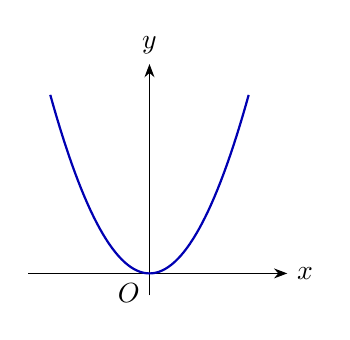
\begin{tikzpicture}[x=0.7cm,y=0.7cm,>=Stealth]
\draw[->](-2.2,0)--(2.5,0)node[right]{$x$};
\draw[->](0,-0.4)--(0,3.8)node[above]{$y$};
\node[below left]at(0,0){$O$};
\draw[thick,blue!70!black,domain=-1.8:1.8,samples=65]plot(\x,{\x*\x});
\end{tikzpicture}
\end{column}
\begin{column}{0.57\textwidth}
\renewcommand{\arraystretch}{1.65}
\begin{tabular}{@{}ll@{}}
定义域 & \Gap{2.8cm}{$\mathbb R$}\\
值域 & \Gap{2.8cm}{$[0,+\infty)$}\\
奇偶性 & \Gap{2.8cm}{偶函数}\\
单调性 & 在 $(-\infty,0]$ 上\Gap{1.4cm}{递减}，\\
 & 在 $[0,+\infty)$ 上\Gap{1.4cm}{递增}。
\end{tabular}
\end{column}
\end{columns}
\Reveal{两个区间分别表述；不能说它在整个 $\mathbb R$ 上递增或递减。}
\end{frame}

% 来源：微信图片_20261112170318_508_20.jpg；五个幂函数表中的 y=x^3。
\begin{frame}[t]{幂函数图像与性质：$y=x^3$}
\large
\begin{columns}[c,onlytextwidth]
\begin{column}{0.40\textwidth}\centering
\begin{tikzpicture}[x=0.7cm,y=0.7cm,>=Stealth]
\draw[->](-2.2,0)--(2.5,0)node[right]{$x$};
\draw[->](0,-2.2)--(0,2.5)node[above]{$y$};
\node[below right]at(0,0){$O$};
\draw[thick,blue!70!black,domain=-1.25:1.3,samples=65]plot(\x,{\x*\x*\x});
\end{tikzpicture}
\end{column}
\begin{column}{0.57\textwidth}
\renewcommand{\arraystretch}{1.65}
\begin{tabular}{@{}ll@{}}
定义域 & \Gap{2.6cm}{$\mathbb R$}\\
值域 & \Gap{2.6cm}{$\mathbb R$}\\
奇偶性 & \Gap{2.6cm}{奇函数}\\
单调性 & 在 $\mathbb R$ 上单调\Gap{1.6cm}{递增}。
\end{tabular}
\end{column}
\end{columns}
\end{frame}

% 来源：微信图片_20261112170318_508_20.jpg；五个幂函数表中的 y=x^(1/2)。
\begin{frame}[t]{幂函数图像与性质：平方根函数}
\large
\begin{columns}[c,onlytextwidth]
\begin{column}{0.40\textwidth}\centering
$y=\sqrt{x}$\par
\begin{tikzpicture}[x=0.7cm,y=0.7cm,>=Stealth]
\draw[->](-0.4,0)--(4.0,0)node[right]{$x$};
\draw[->](0,-0.4)--(0,3.0)node[above]{$y$};
\node[below left]at(0,0){$O$};
\draw[thick,blue!70!black,domain=0:1.85,samples=65]plot({\x*\x},\x);
\end{tikzpicture}
\end{column}
\begin{column}{0.57\textwidth}
\renewcommand{\arraystretch}{1.65}
\begin{tabular}{@{}ll@{}}
定义域 & \Gap{2.8cm}{$[0,+\infty)$}\\
值域 & \Gap{2.8cm}{$[0,+\infty)$}\\
奇偶性 & \Gap{2.8cm}{非奇非偶函数}\\
单调性 & 在 $[0,+\infty)$ 上\Gap{1.4cm}{递增}。
\end{tabular}
\end{column}
\end{columns}
\Reveal{定义域不关于原点对称；定义域与值域都包含 $0$。}
\end{frame}

% 来源：微信图片_20261112170318_508_20.jpg；五个幂函数表中的 y=1/x。
\begin{frame}[t]{幂函数图像与性质：反比例函数}
\large
\begin{columns}[c,onlytextwidth]
\begin{column}{0.40\textwidth}\centering
$y=\dfrac1x$\par
\begin{tikzpicture}[x=0.55cm,y=0.55cm,>=Stealth]
\draw[->](-3.2,0)--(3.5,0)node[right]{$x$};
\draw[->](0,-3.2)--(0,3.5)node[above]{$y$};
\node[below left]at(0,0){$O$};
\draw[thick,blue!70!black,domain=0.32:3.1,samples=70]plot(\x,{1/\x});
\draw[thick,blue!70!black,domain=-3.1:-0.32,samples=70]plot(\x,{1/\x});
\end{tikzpicture}
\end{column}
\begin{column}{0.57\textwidth}
\renewcommand{\arraystretch}{1.65}
\begin{tabular}{@{}ll@{}}
定义域 & \Gap{2.8cm}{$\mathbb R\setminus\{0\}$}\\
值域 & \Gap{2.8cm}{$\mathbb R\setminus\{0\}$}\\
奇偶性 & \Gap{2.8cm}{奇函数}\\
单调性 & 在 $(-\infty,0)$ 上\Gap{1.4cm}{递减}，\\
 & 在 $(0,+\infty)$ 上\Gap{1.4cm}{递减}。
\end{tabular}
\end{column}
\end{columns}
\Reveal{只能说在两个区间上分别递减，不能说在整个定义域上递减。}
\end{frame}

% 来源：微信图片_20261112170325_509_20.jpg；n次方根的概念及个数表。
\begin{frame}[t]{$n$ 次方根的概念}
\large
设 $n>1$ 且 $n\in\mathbb N^*$。若 $x^n=a$，则 $x$ 叫作 $a$ 的 \Gap{2.0cm}{$n$ 次方根}。
\par\vspace{0.3cm}
\renewcommand{\arraystretch}{1.6}
\begin{tabular}{@{}c|c|l@{}}
$n$ 的奇偶性 & $a$ 的范围 & 实数根的情况\\\hline
$n$ 为奇数 & 任意实数 $a$ & 有\Gap{1.3cm}{一个}，记为\Gap{2.0cm}{$\sqrt[n]{a}$}。\\
$n$ 为偶数 & $a>0$ & 有两个，互为\Gap{1.6cm}{相反数}。\\
$n$ 为偶数 & $a=0$ & 只有\Gap{1.4cm}{$0$}。\\
$n$ 为偶数 & $a<0$ & \Gap{2.5cm}{没有实数根}。
\end{tabular}
\Reveal{当 $n$ 为偶数且 $a>0$ 时，两根记为 $\pm\sqrt[n]{a}$。}
\end{frame}

% 来源：微信图片_20261112170325_509_20.jpg；根式的名称、根式性质。
\begin{frame}[t]{根式的名称与性质}
\large
设 $n\ge2$ 为整数。
\begin{enumerate}
\item 式子 $\sqrt[n]{a}$ 叫作根式；$n$ 叫作\Gap{2.0cm}{根指数}，$a$ 叫作\Gap{2.0cm}{被开方数}。
\item 当根式有意义时，$\bigl(\sqrt[n]{a}\bigr)^n=$\Gap{1.8cm}{$a$}。
\item 对任意实数 $a$，若 $n$ 为奇数，$\sqrt[n]{a^n}=$\Gap{1.8cm}{$a$}。
\item 对任意实数 $a$，若 $n$ 为偶数，$\sqrt[n]{a^n}=$\Gap{1.8cm}{$|a|$}。
\item $|a|=\begin{cases}\Gap{1.2cm}{$a$},&a\ge0,\\[0.1cm]\Gap{1.2cm}{$-a$},&a<0.\end{cases}$
\end{enumerate}
\Reveal{偶次根式表示非负的算术根；尤其要记住 $\sqrt{a^2}=|a|$。}
\end{frame}

% 来源：微信图片_20261112170325_509_20.jpg；负分数指数所用的负指数约定，补足零/负整数指数的必要条件。
\begin{frame}[t]{零指数与负整数指数}
\large
\begin{enumerate}
\item 零指数幂：$a^0=$\Gap{1.8cm}{$1$}，条件是\Gap{2.7cm}{$a\ne0$}。
\item 设 $n\in\mathbb N^*$，$a\ne0$，则 $a^{-n}=$\Gap{3.0cm}{$\dfrac1{a^n}$}。
\item 负指数表示取\Gap{1.8cm}{倒数}，不表示在结果前添加负号。
\item $0$ 的负整数指数幂\Gap{2.5cm}{没有意义}。
\end{enumerate}
\Reveal{本课程中 $0^0$ 无意义；非零数的零次幂才等于 $1$。}
\end{frame}

% 来源：微信图片_20261112170325_509_20.jpg；分数指数幂的意义与0的分数指数幂。
\begin{frame}[t]{分数指数幂的意义}
\large
设 $a>0$，$m,n\in\mathbb N^*$，且 $n>1$。
\begin{enumerate}
\item 正分数指数幂：$a^{\frac mn}=$\Gap{3.0cm}{$\sqrt[n]{a^m}$}。
\item 负分数指数幂：$a^{-\frac mn}=$\Gap{2.5cm}{$\dfrac1{a^{m/n}}$}$=$\Gap{2.5cm}{$\dfrac1{\sqrt[n]{a^m}}$}。
\item $0$ 的正分数指数幂等于\Gap{1.5cm}{$0$}；$0$ 的负分数指数幂\Gap{2.3cm}{没有意义}。
\end{enumerate}
\Reveal{本页根式与分数指数互化按正底数表述；不能把负底数直接套入。}
\end{frame}

% 来源：微信图片_20261112170325_509_20.jpg；有理、无理与实数指数幂及运算性质。
\begin{frame}[t]{实数指数幂的运算性质}
\large
一般地，$a^\alpha$（$a>0$，$\alpha$ 是无理数）是一个确定的\Gap{1.6cm}{实数}。
\par\vspace{0.25cm}
设 $a,b>0$，$r,s\in\mathbb R$，则
\[
\begin{aligned}
a^r\cdot a^s&=\Gap{2.9cm}{$a^{r+s}$},\\[0.6em]
(a^r)^s&=\Gap{2.9cm}{$a^{rs}$},\\[0.6em]
(ab)^r&=\Gap{2.9cm}{$a^rb^r$}.
\end{aligned}
\]
\Reveal{同底相乘指数相加，幂的乘方指数相乘；这些规则统一在正底数下使用。}
\end{frame}

% 来源：微信图片_20261112170330_511_20.jpg；指数函数的一般形式与底数条件。
\begin{frame}[t]{指数函数的形式与底数条件}
\large
\begin{enumerate}
\item 指数函数的一般形式为 $y=a^x$，底数条件是\Gap{2.1cm}{$a>0$}且\Gap{2.1cm}{$a\ne1$}。
\item 其中，$a$ 是\Gap{1.8cm}{常数}，$x$ 是\Gap{2.0cm}{自变量}。
\item 指数函数的自变量在\Gap{2.0cm}{指数}位置；幂函数的自变量在\Gap{2.0cm}{底数}位置。
\end{enumerate}
\Reveal{识别时核对完整形式，底数的两个条件都不能漏。}
\end{frame}

% 来源：微信图片_20261112170330_511_20.jpg；指数函数两类图像、定义域、值域、定点。
\begin{frame}[t]{指数函数：图像、范围与定点}
\large
\begin{columns}[T,onlytextwidth]
\begin{column}{0.47\textwidth}\centering
$a>1$\par
\begin{tikzpicture}[x=0.72cm,y=0.52cm,>=Stealth]
\draw[->](-2.5,0)--(2.5,0)node[right]{$x$};
\draw[->](0,-0.3)--(0,4.7)node[above]{$y$};
\node[below left]at(0,0){$O$};
\draw[thick,blue!70!black,domain=-2.3:2.1,samples=70]plot(\x,{pow(2,\x)});
\fill(0,1)circle(1.5pt);
\end{tikzpicture}
\end{column}
\begin{column}{0.47\textwidth}\centering
$0<a<1$\par
\begin{tikzpicture}[x=0.72cm,y=0.52cm,>=Stealth]
\draw[->](-2.5,0)--(2.5,0)node[right]{$x$};
\draw[->](0,-0.3)--(0,4.7)node[above]{$y$};
\node[below left]at(0,0){$O$};
\draw[thick,blue!70!black,domain=-2.1:2.3,samples=70]plot(\x,{pow(2,-\x)});
\fill(0,1)circle(1.5pt);
\end{tikzpicture}
\end{column}
\end{columns}
\par\vspace{0.18cm}
定义域：\Gap{2.2cm}{$\mathbb R$}；\quad 值域：\Gap{3.0cm}{$(0,+\infty)$}。
\par\vspace{0.18cm}
图像过定点\Gap{2.2cm}{$(0,1)$}，即当 $x=0$ 时，$y=$\Gap{1.3cm}{$1$}。
\end{frame}

% 来源：微信图片_20261112170330_511_20.jpg；指数函数单调性、奇偶性、两曲线对称性。
\begin{frame}[t]{指数函数：单调性、奇偶性与对称性}
\large
设 $y=a^x$，其中 $a>0$ 且 $a\ne1$。
\begin{enumerate}
\item 当 $a>1$ 时，在 $\mathbb R$ 上单调\Gap{2.0cm}{递增}。
\item 当 $0<a<1$ 时，在 $\mathbb R$ 上单调\Gap{2.0cm}{递减}。
\item 指数函数是\Gap{3.5cm}{非奇非偶函数}。
\item 函数 $y=a^x$ 与 $y=a^{-x}$ 的图像关于\Gap{2.5cm}{$y$ 轴}对称。
\end{enumerate}
\Reveal{判断单调性先看底数范围；两条曲线互相对称，不代表其中一条是偶函数。}
\end{frame}


\begin{frame}[t]{最后核对自己的遗漏}
\begin{enumerate}
\item 回看刚才填错或没有填出的空，圈出对应页号。
\item 把该条知识的完整结论与条件补写一遍。
\item 遮住答案，再回到挖空页填写一次。
\end{enumerate}
\par\vspace{0.6cm}
\textbf{检查重点：}符号、量词、范围、端点、非零条件与等号。
\end{frame}
\end{document}
